\subsection{Water Disaggregation and Constraints}
Aggregated water usage displays different characteristics. 
The total water consumption is zero most of the time.
Whenever a water device is used, water is consumed intensively for a period of time,
which forms a series of user behavior. 
For instance, a person may use the toilet in the bathroom first, 
then wash hands in the sink and take a shower afterwards. 
This series of events highly affects electricity usage as well. 
When the person enters into the bathroom, the light in the bathroom is turned on. 
After using the bathroom, the person leaves and turns the light off. 
Moreover, we observe that the usage of toilet is usually accompanied by
sink usage afterwards. 

In this subsection, we apply the semi-supervised multivariate piecewise motif mining 
to water data. 
First, we apply similar feature extraction to water data set,
and obtain the water flow rate level for each device.
Table \ref{table_resultStudy10Water} lists the water consumption rate for each device.
These water devices are usually turned on in a short period of duration, 
and stay off during much longer time. 

Then we utilize multivariate piecewise motif mining approach to 
water disaggregation. 
%The disaggregation results are shown in Table \ref{table_resultStudy10Water}.
\begin{table*}[!t]
\renewcommand{\arraystretch}{1.3}
\caption{Water Flow Rate Levels of Water End Uses and Disaggregation Results}
\label{table_resultStudy10Water}
\centering
\begin{tabular}{|c|c|c|c|c|c|c|}
\hline
\multirow{2}{*}{Device} & \multirow{2}{*}{Hot water} & \multirow{2}{*}{Cold water} & \multirow{2}{*}{Duration} &  \multirow{2}{*}{Precision} & \multirow{2}{*}{Recall} &  \multirow{2}{*}{F-measure}\\
           &  (liter/min) & (l/min*10000)& (second) & & & \\
\hline
\hline
Shower & $\alpha \in (1822, 1986)$ & $1904-\alpha$& on: 2 & 0.999 & 0.972 & 0.986 \\
\hline
Washing Machine & $\alpha \in (1988, 2276)$  & $2132-\alpha$ & on: 5& 0.997  & 0.969 & 0.983\\
\hline
DownToilet & 0 & (1270, 1400) & whole: 50& NA & NA & NA\\
\hline
UpToilet & 0 & (1480, 1700) & whole: 50& NA & NA & NA \\
%\hline
%KitchenSink &  $ \alpha \in (0, 57) $ & 57- $\alpha$ & 2& & & \\
%\hline
%UpSink & 34 & 160 & 2& & & \\
%\hline
%DownSink & 57  & 80 & 2& & & \\
%\hline
%Dish Washer & 34 & -11 & 2& & & \\
\hline
\end{tabular}
\end{table*}

For shower and washing machine, 
the total flow rate of hot and cold water is high,  nearly 0.2 Liter/Minute. 
Therefore by only searching the 
total hot and cold water flow rate, we can identify these two devices. 
The event of shower usually lasts for more than one minute. 
But the washing machine uses water for less than one minute, 
repeating for $6-9$ times. 
Both the shower and washing machine use 
hot water and cold water. 
However, the washing machine only uses hot water for the 
first one or two times. Then in the rest, 
only cold water is used. 
Whenever the washing machines starts, 
the power consumption starts as well. 

\begin{figure*}[!t]
        \centering{
                \begin{tabular}{cc}
                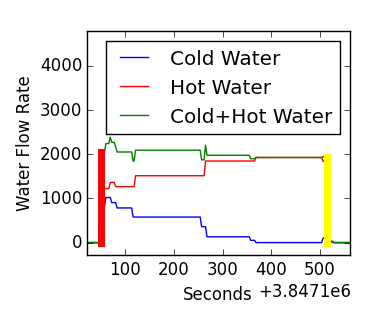
\includegraphics[width=0.5\textwidth]{multidisaggfig/showerFitted.png}&
                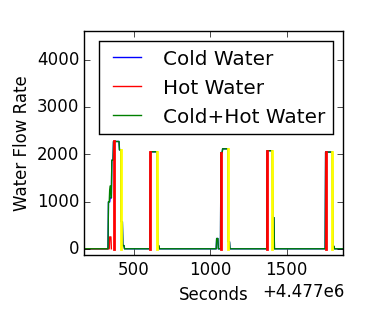
\includegraphics[width=0.5\textwidth]{multidisaggfig/washingMachineWaterFitted.png}\tabularnewline
                (a) & (b)\tabularnewline
                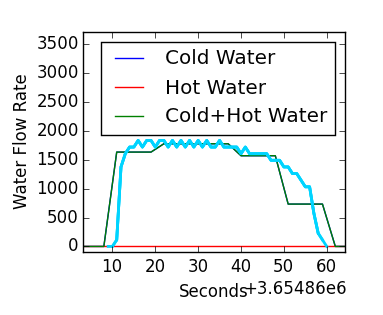
\includegraphics[width=0.5\textwidth]{multidisaggfig/UpToiletFitted.png}&
                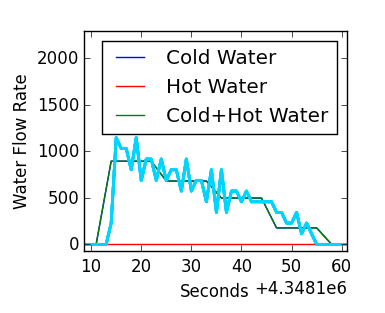
\includegraphics[width=0.5\textwidth]{multidisaggfig/DownToiletFitted.png}
                \tabularnewline
                 (c) & (d)\tabularnewline
                \end{tabular}
                }
        \caption{
        X-axis is the duration to a specific time in seconds, Y-axis is water flow rate in 10000*liter/minute. 
	(a) and (b) denote the water disaggregation of shower and washing machine. The fitted red line denotes the on event of water, and the fitted yellow line denotes the off event of water. 
	(c) and (d) are the disaggregated two toilets of complete usage cycle by dynamic time warping subsequence search. 
	}
        \label{fig_waterDisaggResults}
\end{figure*}
%Figure \ref{fig_waterDisaggResults} (a) and (b) display the water usage of shower and washing machine. 
With piecewise motif mining to the water usage, 
shower and washing machine are disaggregated as in Figure \ref{fig_waterDisaggResults} (a) and (b).
But with variable water flow rate water use end such as toilet, 
piecewise motif mining has limitation on handling with it. 
Therefore we use dynamic time warping subsequence~\cite{rakthanmanon2012searching} search as an complementary to discover them.  
For the two toilets, we apply dynamic time warping to match the time series.
The results of toilet water usage are shown in Figure \ref{fig_waterDisaggResults} (c) and (d). 

%There are totally three sinks in the house, namely up sink, down sink and kitchen sink. 
%People may use sinks with only hot water or cold water, or both hot and cold water. 
%The water usage may be large or small. 
%In this case, it is hard to distinguish these three sinks. 
%However, by observing the water usage of up sink and down sink. 
%We find that there's correlation between the down sink and the down toilet, 
%up sink and up toilet. 
%Figure \ref{fig_ToiletSinkCorrelation} (a) and (b) show that the toilet and sink start almost at the same time, 
%or end at the same time. 
We can see that multivariate piecewise motif mining is capable of 
disaggregating water use ends which has sharp on/off water flow rate. 
But it has limitations in dealing with water use end with irregular water use patterns 
such as toilets and sinks. 
Since the water usage of toilets is relatively fixed if using alone, 
some toilet water usages can be disaggregated by dynamic time warping subsequence search 
which was researched in \cite{nguyen2013development}. 

